\chapter{SYSTEM WORKFLOW}

\section{Introduction}

The proposed pneumatic tip-growing robot integrates a flexible eversion mechanism, four-tendon steering, pneumatic actuation, camera-based object detection, and ROS 2-based control. The system workflow describes how these components interact to support forward growth and directional steering.

The overall system is divided into mechanical, pneumatic, perception, planning, and control functions. The pneumatic subsystem supports the extension of the flexible tube, while four servo motors located at the base station control the steering tendons. A camera positioned near the growing tip captures images of the surrounding environment, and a pretrained YOLO model processes the images to detect objects belonging to its supported classes.

ROS 2 provides the communication framework connecting the perception and control components. The resulting architecture allows each subsystem to be developed and tested independently before integration.

\section{Overall System Operation}

The system operates through a sequence of image acquisition, object detection, path planning, tendon steering, and pneumatic growth control.

Initially, the pneumatic subsystem supplies air to the flexible tube to initiate or maintain eversion. At the same time, the camera captures images of the environment ahead of the growing tip. The object detection node processes these images using the pretrained YOLO model and produces detection results.

The path-planning component interprets the available environmental information and determines a desired movement direction according to the implemented navigation strategy. The steering controller converts this direction into coordinated commands for the four servo motors.

The pneumatic controller regulates the growth command according to the intended operating sequence and available pressure feedback. During operation, updated camera images can provide further information for subsequent steering and planning decisions.

\section{Pneumatic Growth Mechanism}

The pneumatic subsystem provides the pressure required to extend the flexible growing tube through eversion. An air pump or compressor supplies air through the pneumatic circuit, which may include a regulator, control valve, pressure sensor, and connecting tubing.

The pressure regulator helps establish the intended operating pressure, while the control valve manages the air supply according to the growth command. A pressure sensor can provide feedback to the controller for monitoring operating conditions.

The flexible tube advances as material everts at the growing tip. The actual growth rate and stability depend on the tube material, geometry, applied pressure, friction, and interaction with the surrounding environment.

The pneumatic subsystem is therefore treated as a separate control function from the tendon-steering mechanism, although both must operate in coordination during robot movement.

\section{Four-Tendon Steering Mechanism}

Directional control is provided by four axial tendons arranged around the flexible tube. Each tendon is connected to a servo-actuation mechanism positioned at the base station.

The tendons are arranged to provide steering authority in different directions in the X--Y plane. Coordinated tendon displacement and tension produce bending of the steering region near the growing tip. The direction and magnitude of bending depend on the tendon arrangement, attachment geometry, tension, and mechanical properties of the flexible structure.

The steering controller calculates the required tendon commands from the desired direction. These commands are transmitted to the servo-control hardware, which positions the servo motors accordingly.

Because the tube continues to grow during operation, the tendon mechanism must also accommodate cable payout and maintain appropriate routing and tension. The relationship between servo movement and actual tip direction must be calibrated on the physical mechanism.

\section{Camera-Based Object Detection}

The perception subsystem uses a camera mounted near the growing tip to capture images of the surrounding environment. The camera stream is made available to a ROS 2 node for image processing.

The object detection node converts each image into the format required by the selected pretrained YOLO inference interface. The image is resized or letterboxed as necessary, and the model performs inference to identify supported object classes.

The resulting detections contain class labels, confidence scores, and bounding-box coordinates. These results provide visual information about objects in the camera's field of view.

The perception subsystem does not independently determine a safe trajectory. Instead, its output is supplied to the path planner, which interprets the detections according to the navigation strategy. If accurate obstacle distance is required, additional depth sensing, calibration, or geometric estimation may be required.

\section{ROS 2 Path Planning and Control}

ROS 2 connects the perception, planning, and actuation components through a modular software architecture.

The camera node publishes image messages, and the object detection node processes the incoming images. The path planner receives the detection information and determines a desired direction or path based on the available environmental representation and navigation logic.

The steering controller converts the desired direction into commands for the four tendon actuators. The servo-control interface sends these commands to the base-mounted servo motors through the embedded hardware controller.

A separate growth-control function manages the pneumatic valve and air supply. Pressure feedback, when available, can be used to monitor the pneumatic subsystem and support appropriate control or safety responses.

The separation of these functions simplifies software development and allows the perception, planning, steering, and growth components to be tested independently.

Figure~\ref{fig:system_architecture} illustrates the overall ROS~2 software architecture and hardware interface for the proposed growing robot.

\begin{figure}[H]
    \centering
    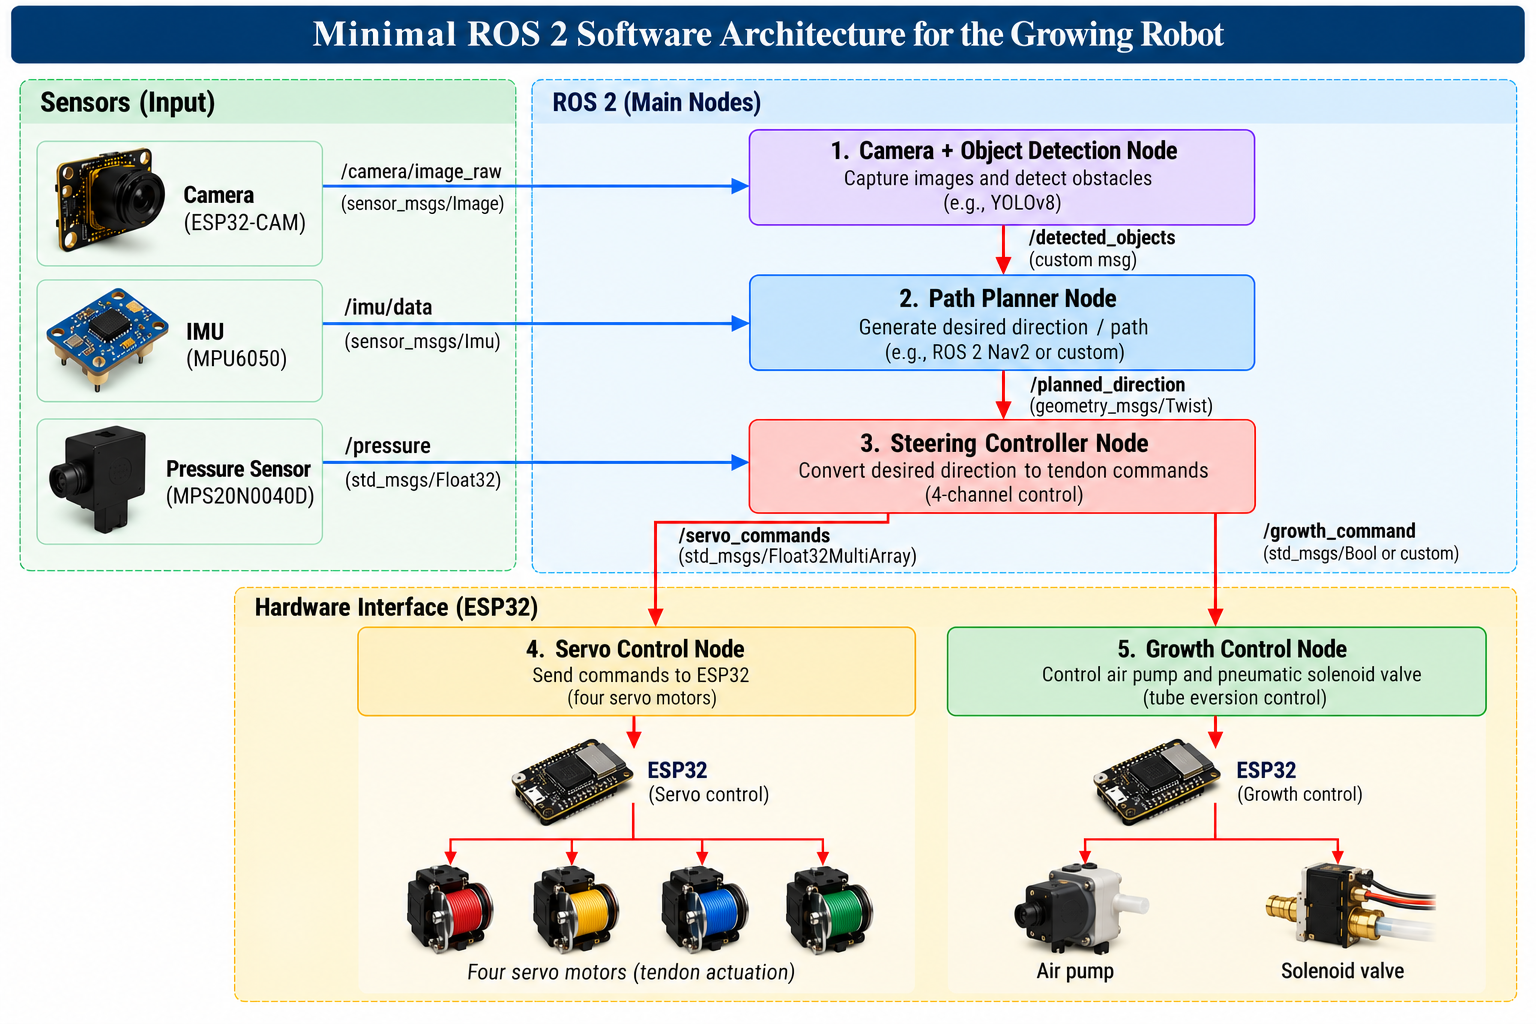
\includegraphics[width=0.95\textwidth]{img/5_architecture.png}
    \caption[ROS 2 Architecture and Hardware Interface]{ROS 2 Software Architecture and Hardware Interface for the Growing Robot}
    \label{fig:system_architecture}
\end{figure}

\section{Integrated System Workflow}

The complete proposed workflow consists of the following steps:

\begin{enumerate}
    \item \textbf{System initialization:} Initialize the camera, ROS 2 nodes, embedded controller, servo interface, and pneumatic control components.
    \item \textbf{Pneumatic growth:} Supply regulated air to initiate or maintain eversion of the flexible tube.
    \item \textbf{Image acquisition:} Capture images of the environment using the tip-mounted camera.
    \item \textbf{Image preprocessing:} Convert the camera image into the input format required by the pretrained YOLO model.
    \item \textbf{Object detection:} Run inference and obtain supported object classes, confidence scores, and bounding boxes.
    \item \textbf{Path planning:} Interpret the detection results and determine a desired movement direction according to the implemented navigation strategy.
    \item \textbf{Tendon steering:} Convert the desired direction into coordinated commands for the four servo motors.
    \item \textbf{Growth coordination:} Manage pneumatic growth while ensuring that tendon movement and cable payout remain compatible with continued eversion.
    \item \textbf{Repeated perception:} Acquire updated images and repeat the planning and steering process as required.
\end{enumerate}

This workflow describes the intended system operation. The actual timing, control frequency, and feedback behavior will depend on the implemented hardware and software.

\section{System Feedback and Safety}

Feedback is important for maintaining controlled operation. A pressure sensor can monitor pneumatic pressure, while an IMU or other suitable sensing arrangement may provide information about the robot's orientation or movement. Camera observations can provide additional environmental information.

The available measurements should be used to detect conditions such as excessive pressure, stalled growth, unexpected steering response, or loss of reliable perception. Appropriate limits and shutdown behavior should be established before physical testing.

The pneumatic system should include pressure regulation and suitable overpressure protection. Servo commands and tendon tension should also be limited to avoid damaging the flexible tube or steering mechanism.

The feedback architecture should be expanded according to the sensors actually installed and validated. The presence of a sensor or software node alone does not establish that the robot has closed-loop steering or autonomous obstacle avoidance.